\documentclass[12pt]{article}
\usepackage[brazil]{babel} % idioma PT-BR
\usepackage{indentfirst} % esse pacote aplica a indentação
\usepackage[export]{adjustbox}
%\setlength{\parindent}{1cm} % este comando altera a indentação do parágrafo
%\setlength{\parskip}{.5cm} % este comando altera o espaço entre parágrafos
\usepackage{setspace} % esse pacote altera o espaçamento entre linhas
\usepackage[a4paper, left=3cm, right=2cm, top=3cm, bottom=2cm]{geometry} % este pacote altera a margem do documento
\usepackage[usenames, dvipsnames]{xcolor} % modifica as cores
\usepackage{graphicx} % este pacote permite adicionar figuras
\usepackage{float} % força o posicionamento da figura
\usepackage{amsmath} % Modo matemático
\usepackage{url}
\usepackage{csvsimple} 


\begin{document}
    \begin{figure}
        \centering
        
\includegraphics[width=0.35\linewidth]{Figuras/ufsj-logo-2018}
        \\\setlength{\parskip}{1cm}
        \textbf{UNIVERSIDADE FEDERAL DE SÃO JOÃO DEL-REI \\
         DEPARTAMENTO DE CIÊNCIA DA COMPUTAÇÃO\\
         ALGORITMO E ESTRUTURA DE DADOS III}\\
%        Algoritmo e estrutura de dados III 

        \label{fig:ufsj-logo-2018}
    \end{figure}
    
    \author{Gustavo Henriques \\ Matheus N Silva}

    \title{ 
        \vspace{6cm} % adiciona espaço entre parágrafos
		    \textbf{TRABALHO PRATICO 2}
		\vspace{6cm} % adiciona espaço entre parágrafos
	}
	\setstretch{1.5} % define o tamanho do espaçamento de linhas 
    \date{$ $\\ São João del-Rei \\ 2023}
    \maketitle
    \thispagestyle{empty} % remove numeração da pagina
    \newpage
    
    \setcounter{page}{1} % Inicia a ordem de numeração das paginas
    \pagenumbering{Roman} % Estilo de numeração Romana
    \listoffigures
    \listoftables
    \newpage

    \tableofcontents % Cria sumário
    \newpage
    
    
    \setcounter{page}{1} % Inicia a ordem de numeração das paginas
    \pagenumbering{arabic} % Estilo de numeração Arábica
    \section{INTRODUÇÃO} % Titulo da secção
        \subsection{Proposta}
        Este trabalho propõe um problema que consiste em ajudar Harry Potter a percorrer 
        um grid com poções e monstros, de forma a chegar ao seu destino gastando a menor 
        quantidade de energia possível.
            
        \subsection{Objetivo}
            Nosso objetivo é analisar os possíveis caminhos que ele pode seguir e 
            determinar a quantidade de energia com a qual ele deve começar para manter 
            um nível positivo de energia durante todo o percurso. A fim de auxiliar na 
            resolução do problema, podemos reformulá-lo de maneira mais formal da seguinte 
            forma:
            Dada uma matriz de dimensão RxC, com pesos positivos ou negativos em cada uma 
            de suas células, encontrar um caminho da posição (1,1) até a posição (R,C) de 
            modo que a soma mínima de energia ao longo do caminho seja a maior possível.

            Podemos abordar esse problema de maneira recursiva, em que a soma de uma 
            célula (i,j) em um caminho é igual ao seu peso mais o peso da célula anterior 
            no caminho. Podemos utilizar isso para construir uma solução de força bruta 
            para o problema, no entanto, como veremos adiante, essa solução não é eficiente 
            e não será útil para Harry, dependendo do tamanho do grid. Para melhorar isso, 
            ao observarmos a árvore de recursão do problema, percebemos que alguns problemas 
            se repetem, o que sugere a possibilidade de uma solução utilizando programação 
            dinâmica. Conforme veremos mais adiante, isso de fato é possível, permitindo-nos 
            desenvolver uma solução eficiente que será útil para Harry, mesmo em um grid de 
            grande tamanho.
     
    \newpage
    \section{IMPLEMENTAÇÃO}
        \subsection{Força bruta}
            Ao analisar o problema, a solução mais simples que podemos considerar é examinar 
            cada caminho e determinar qual deles requer o menor consumo inicial de energia. 
            Assim, a solução 2 do nosso trabalho utiliza essa abordagem de força bruta.

            Para implementar esse método, podemos aproveitar a natureza recursiva do problema 
            e construir uma função recursiva. Além disso, utilizaremos um TAD no formato de 
            uma matriz com dimensões RxC, que armazenará cada elemento do grid, bem como o 
            valor necessário para retornar a energia mínima que Harry precisa para atravessar 
            o grid.
            
            A função inicia na posição inicial do grid e chama a si mesma recursivamente para 
            as posições adjacentes à célula atual. Ela soma o peso da célula atual com o peso 
            da célula anterior e armazena o menor valor encontrado ao longo do caminho. 
            No caso base, quando chegamos à última célula do grid, verificamos se o valor mínimo 
            do caminho atual é maior do que os valores dos caminhos anteriores, pois procuramos 
            o caminho com o valor mínimo máximo.
            
            Essa função segue a árvore de recursão abaixo, onde cada ramo representa um caminho 
            diferente.
            
            \begin{figure}[h]
                \centering
                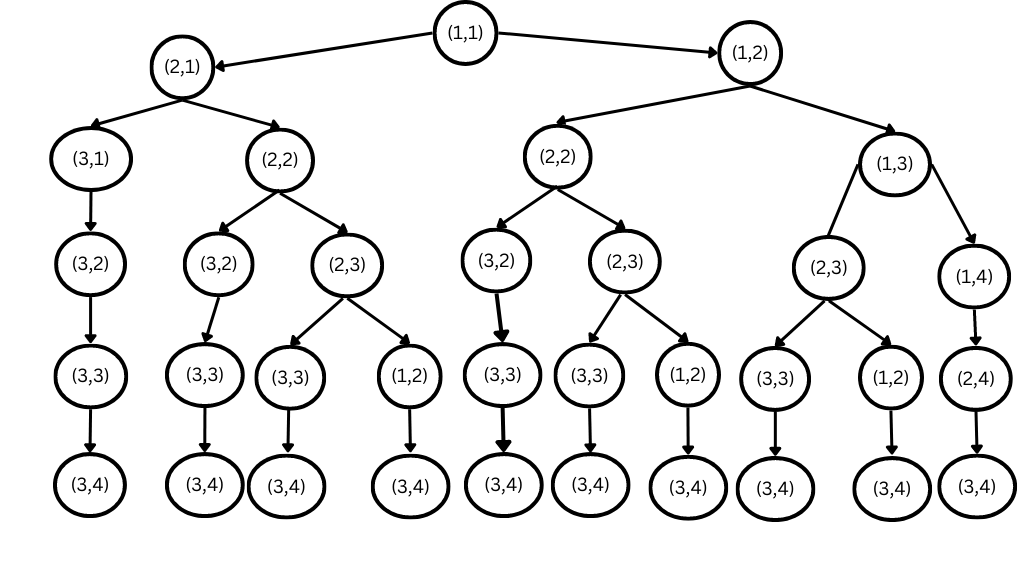
\includegraphics[width=0.75\linewidth]{Figuras/arvoreRecursao.png}\\
                \caption{Árvore de recursão de um grid de dimensões 3x4}
                \label{fig:Arvore de recursão}
            \end{figure}
            
            \subsubsection{Complexidade da solução por força bruta}
                Conforme esperado de uma solução de força bruta, essa estratégia é extremamente 
                ineficiente em termos de tempo de execução. Ao analisar a complexidade da função, 
                percebemos que ela percorre todas as posições do grid, e em cada posição pode 
                fazer até duas chamadas recursivas. Portanto, a complexidade é exponencial. 
                Ao testar a função várias vezes com as diretivas "rusage" e "gettimeofday" em C, 
                e usando o R para analisar os dados gerados, podemos observar que o tempo de 
                execução cresce de forma exponencial à medida que aumentamos o tamanho da entrada.

                \begin{figure}[h]
                    \centering
                    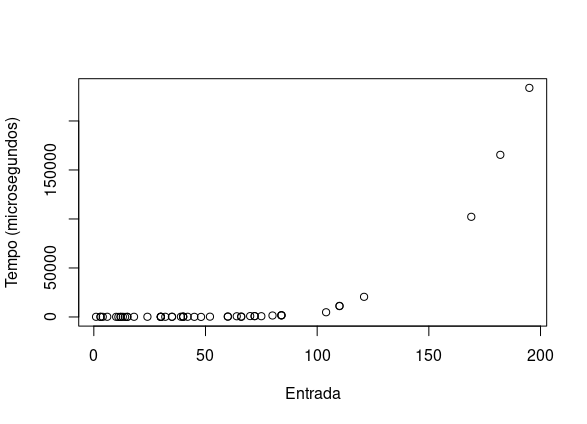
\includegraphics[width=0.9\linewidth]{Figuras/graficoForcaBruta.png}\\
                    \caption{Gráfico da solução utilizando força bruta}
                    \label{fig:grafico forca bruta}
                    \textit{Obs.: Esse gráfico foi construido com base na função gettimeofday}
                \end{figure}

                Podemos observar que, com entradas acima de 100, ou seja, um grid com dimensões 
                superiores a 10x10, o tempo necessário para calcular a energia aumenta rapidamente. 
                Durante nossos testes, com um grid de dimensões 20x20, não obtivemos a resposta 
                mesmo após esperar por 5 minutos.
        \newpage
        \subsection{Programação dinâmica}
            Ao observarmos a imagem da árvore de recursão da solução de força bruta, podemos notar 
            que alguns ramos se repetem, o que nos indica a possibilidade de uma solução utilizando 
            programação dinâmica. No entanto, essa solução não é tão evidente. Se tentarmos apenas 
            começar na posição inicial e escolher a próxima célula do caminho buscando maximizar a 
            soma, como em um problema de encontrar a maior distância, perceberemos que essa abordagem 
            não satisfaz o princípio da otimalidade, que é um dos requisitos para construir uma 
            solução com programação dinâmica.

            Para alcançar uma solução ótima utilizando esse método, devemos pensar no problema de 
            baixo para cima. Basicamente, precisamos determinar a energia mínima necessária em cada 
            célula, de forma a chegar nela com uma energia mínima de 1. Assim, começando da última 
            célula do grid, podemos verificar qual deveria ser a energia necessária para alcançá-la. 
            Se essa energia for negativa, por exemplo, -5, devemos chegar na célula com uma energia 
            de 6. Para chegar nessa célula, temos duas opções: vindo de cima ou vindo da esquerda. 
            Ao analisarmos essas posições, devemos verificar se seus pesos são suficientes para 
            atingir a célula atual. No exemplo dado, como precisamos chegar com energia 6, as células 
            adjacentes devem ter uma energia de pelo menos 6, e nesse caso podemos chegar nelas com 
            a energia mínima de 1. Por outro lado, se o peso da célula adjacente não for suficiente, 
            isso significa que devemos chegar nela com um peso que permita atingir a célula atual com 
            o peso necessário. No exemplo mencionado, se uma célula adjacente tiver peso 4, significa 
            que precisamos chegar nela com peso 2, para que possamos alcançar a célula atual com o 
            peso necessário.
            
            Para implementar isso, utilizaremos uma estrutura de dados no formato de uma tabela, 
            com as mesmas dimensões do grid. Cada posição (i, j) da tabela nos fornecerá o peso 
            mínimo necessário para chegar à posição (i, j) do grid, de modo que a energia de Harry 
            permaneça positiva durante todo o caminho.
            
            Iniciaremos na posição (R, C) e percorreremos o grid de baixo para cima, analisando cada 
            coluna de cada vez, o que nos permitirá preencher a tabela com segurança. O resultado para 
            determinar a energia inicial será armazenado na posição inicial da tabela. Essa é a solução 
            1 do nosso trabalho.

            \subsubsection{Complexidade da solução por programação dinâmica}
                A solução apresentada com programação dinâmica é consideravelmente melhor do que a 
                solução de força bruta, com uma complexidade de O(R*C), pois percorre cada elemento do 
                grid realizando operações constantes.

                Assim como na solução de força bruta, realizamos testes e utilizamos o R para analisar 
                os resultados, embora o gráfico dos testes não ilustre tão claramente a ordem de 
                complexidade como na solução anterior.

                \begin{figure}[h]
                    \centering
                    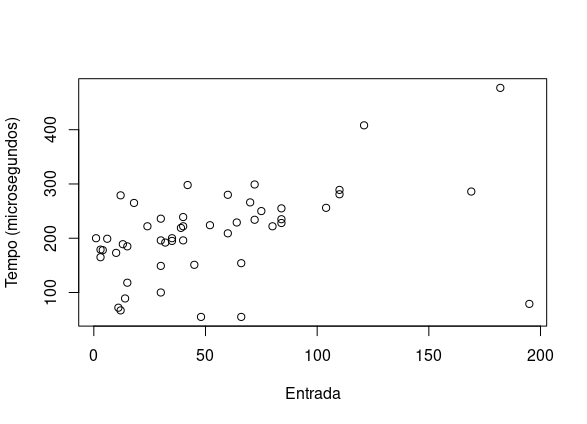
\includegraphics[width=0.9\linewidth]{Figuras/graficoPD1.png}\\
                    \caption{Gráfico da solução utilizando programação dinâmica}
                    \label{fig:grafico programacao dinamica }
                    \textit{Obs.: Esse gráfico foi construido com base na função gettimeofday}
                \end{figure}

                Isso pode não ter ficado claro, pois o algoritmo é muito rápido, sendo necessários testes
                grandes, com condições de teste mais rigorosas, considerando a máquina, a memória e outros 
                fatores externos que possam influenciar o tempo de execução. É justamente por causa dessas 
                variáveis que confiamos no cálculo de complexidade para determinar a eficiência da solução.


    \newpage
    \section{AVALIAÇÃO DE RESULTADOS}
        Além da ordem de complexidade, realizamos alguns testes comparando as duas soluções e seu desempenho 
        em casos de teste idênticos, gerados aleatoriamente, com um grid de dimensões máximas de 20x10.

        Abaixo, apresentamos uma tabela comparando os resultados dos algoritmos em vários testes iguais:
       
        \textit{Obs.: As configurações de hardware utilizados para os testes são as seguintes:\\ 
        CPU: Intel i5-10210U, RAM: 8gb - 2333mhz, SO: Ubuntu 22.04.2 lts}
        \begin{table}[h!]
            \centering
            \begin{tabular}{|c|c|c|c|c|c|}
                \hline
                    Resultado & Entrada & Rusage & Gettimeofday & Usuario & Sistema \\ \hline
                    1 & 30 & 1.846.00ms & 207.00ms & 0.00ms & 1846.00ms \\ \hline
                    83 & 80 & 2901.00ms & 1498.00ms & 0.00ms & 2901.00ms \\ \hline
                    1 & 66 & 515.00ms & 138.00ms & 515.00ms & 0.00ms \\ \hline
                    145 & 12 & 1928.00ms & 183.00ms & 0.00ms & 1928.00ms \\ \hline
                    1 & 48 & 455.00ms & 63.00ms & 455.00ms & 0.00ms \\ \hline
                    1 & 40 & 1892.00ms & 252.00ms & 0.00ms & 1892.00ms \\ \hline
                    80 & 3 & 2076.00ms & 180.00ms & 0.00ms & 2076.00ms \\ \hline
                    70 & 60 & 2236.00ms & 521.00ms & 2236.00ms & 0.00ms \\ \hline
                    1 & 182 & 167165.00ms & 165448.00ms & 167165.00ms & 0.00ms \\ \hline
                    1 & 15 & 1591.00ms & 163.00ms & 1591.00ms & 0.00ms \\ \hline
                    17 & 70 & 2774.00ms & 901.00ms & 2774.00ms & 0.00ms \\ \hline
                    1 & 3 & 1617.00ms & 159.00ms & 1617.00ms & 0.00ms \\ \hline
                    1 & 18 & 1885.00ms & 197.00ms & 1885.00ms & 0.00ms \\ \hline
                    1 & 10 & 1581.00ms & 163.00ms & 1581.00ms & 0.00ms \\ \hline
                    1 & 24 & 1844.00ms & 211.00ms & 1844.00ms & 0.00ms \\ \hline
                    122 & 72 & 2493.00ms & 890.00ms & 2493.00ms & 0.00ms \\ \hline
                    76 & 35 & 1552.00ms & 192.00ms & 1552.00ms & 0.00ms \\ \hline
                    15 & 42 & 1787.00ms & 207.00ms & 1787.00ms & 0.00ms \\ \hline
                    1 & 45 & 1048.00ms & 147.00ms & 1048.00ms & 0.00ms \\ \hline
                    1 & 169 & 103638.00ms & 102211.00ms & 103638.00ms & 0.00ms \\ \hline
                    97 & 40 & 2120.00ms & 320.00ms & 0.00ms & 2120.00ms \\ \hline
                    1 & 4 & 1639.00ms & 155.00ms & 1639.00ms & 0.00ms \\ \hline
                    1 & 13 & 1715.00ms & 173.00ms & 0.00ms & 1715.00ms \\ \hline
                    1 & 84 & 3066.00ms & 1620.00ms & 0.00ms & 3066.00ms \\ \hline
                    14 & 75 & 2387.00ms & 772.00ms & 2387.00ms & 0.00ms \\ \hline
                    272 & 30 & 1638.00ms & 225.00ms & 1638.00ms & 0.00ms \\ \hline
                    88 & 110 & 12956.00ms & 11351.00ms & 12956.00ms & 0.00ms \\ \hline
                    100 & 6 & 1850.00ms & 218.00ms & 1850.00ms & 0.00ms \\ \hline
                    1 & 1 & 1906.00ms & 177.00ms & 0.00ms & 1906.00ms \\ \hline
                    1 & 40 & 1775.00ms & 272.00ms & 1775.00ms & 0.00ms \\ \hline
                    38 & 12 & 570.00ms & 57.00ms & 570.00ms & 0.00ms \\ \hline
            \end{tabular}
            \caption{Tabela resultados força bruta}
            \label{Tabela: Forca Bruta}
        \end{table}

        \begin{table}[!ht]
            \centering
            \begin{tabular}{|c|c|c|c|c|c|}
                \hline
                Resultado & Entrada & Rusage & Gettimeofday & Usuario & Sistema \\ \hline
                1 & 30 & 2031.00ms & 236.00ms & 2031.00ms & 0.00ms \\ \hline
                83 & 80 & 1755.00ms & 222.00ms & 1755.00ms & 0.00ms \\ \hline
                1 & 66 & 456.00ms & 55.00ms & 456.00ms & 0.00ms \\ \hline
                145 & 12 & 2170.00ms & 279.00ms & 2170.00ms & 0.00ms \\ \hline
                1 & 48 & 526.00ms & 55.00ms & 526.00ms & 0.00ms \\ \hline
                1 & 40 & 1718.00ms & 196.00ms & 1718.00ms & 0.00ms \\ \hline
                80 & 3 & 1718.00ms & 179.00ms & 1718.00ms & 0.00ms \\ \hline
                70 & 60 & 2130.00ms & 280.00ms & 2130.00ms & 0.00ms \\ \hline
                1 & 182 & 2180.00ms & 477.00ms & 0.00ms & 2180.00ms \\ \hline
                1 & 15 & 1808.00ms & 185.00ms & 0.00ms & 1808.00ms \\ \hline
                17 & 70 & 2253.00ms & 266.00ms & 0.00ms & 2253.00ms \\ \hline
                1 & 3 & 1687.00ms & 165.00ms & 1687.00ms & 0.00ms \\ \hline
                1 & 18 & 2287.00ms & 265.00ms & 2287.00ms & 0.00ms \\ \hline
                1 & 10 & 1734.00ms & 173.00ms & 0.00ms & 1734.00ms \\ \hline
                1 & 24 & 2135.00ms & 222.00ms & 2135.00ms & 0.00ms \\ \hline
                122 & 72 & 1864.00ms & 299.00ms & 1864.00ms & 0.00ms \\ \hline
                76 & 35 & 1733.00ms & 195.00ms & 1733.00ms & 0.00ms \\ \hline
                15 & 42 & 1974.00ms & 298.00ms & 1974.00ms & 0.00ms \\ \hline
                1 & 45 & 1252.00ms & 151.00ms & 1252.00ms & 0.00ms \\ \hline
                1 & 169 & 1820.00ms & 286.00ms & 0.00ms & 1820.00ms \\ \hline
                97 & 40 & 2004.00ms & 222.00ms & 0.00ms & 2004.00ms \\ \hline
                1 & 4 & 1818.00ms & 178.00ms & 1818.00ms & 0.00ms \\ \hline
                1 & 13 & 1815.00ms & 189.00ms & 1815.00ms & 0.00ms \\ \hline
                1 & 84 & 1797.00ms & 228.00ms & 1797.00ms & 0.00ms \\ \hline
                14 & 75 & 2017.00ms & 250.00ms & 2017.00ms & 0.00ms \\ \hline
                272 & 30 & 1758.00ms & 196.00ms & 0.00ms & 1758.00ms \\ \hline
                88 & 110 & 2107.00ms & 289.00ms & 0.00ms & 2107.00ms \\ \hline
                100 & 6 & 1997.00ms & 199.00ms & 0.00ms & 1997.00ms \\ \hline
                1 & 1 & 2027.00ms & 200.00ms & 2027.00ms & 0.00ms \\ \hline
                1 & 40 & 1990.00ms & 239.00ms & 1990.00ms & 0.00ms \\ \hline
                38 & 12 & 692.00ms & 67.00ms & 692.00ms & 0.00ms \\ \hline
            \end{tabular}
            \caption{Tabela resultados programação dinâmica}
            \label{Tabela: Programacao Dinamica}
        \end{table}
        Nos testes realizados com essas entradas, utilizando a diretiva "gettimeofday", o algoritmo de força 
        bruta teve uma média de tempo de 11.332,5 microssegundos, enquanto o algoritmo com programação dinâmica 
        teve uma média de apenas 208,9 microssegundos, considerando entradas menores que 200, que não podem ser 
        consideradas grandes.

        Outra diferença significativa entre o desempenho das duas soluções foi observada durante os testes. 
        Enquanto a solução de força bruta não conseguiu encontrar uma solução para uma entrada de 400, mesmo 
        após 5 minutos, como mencionado anteriormente, o algoritmo com programação dinâmica conseguiu retornar 
        o resultado para uma entrada de 98.565.184 em cerca de 16,19 segundos. Isto é, com uma entrada 245.000 
        vezes maior, o algoritmo de programação dinâmica conseguiu calcular com facilidade uma resposta, enquanto 
        que o algoritmo com força bruta demora vários minutos para calcular uma entrada extremamente menor.
        
        \textit{Obs.: Os demais testes estão contidos na pasta "testes\_tp2" dentro da pasta raiz da aplicação}
    \newpage
    \section{CONCLUSÃO}
        O problema proposto, embora seja complicado e não seja fácil identificar uma solução eficiente imediatamente, 
        possui de fato uma solução rápida que consegue calcular facilmente uma resposta, mesmo para entradas muito 
        grandes. A parte do código neste trabalho foi extremamente simples, com ambas as soluções ocupando poucas 
        linhas e sendo claras e objetivas, o que facilitou o entendimento. A maior dificuldade foi compreender o 
        problema e pensar na solução com programação dinâmica para otimizar os subproblemas e calcular o problema 
        geral com facilidade.

        Ao analisarmos os resultados, pudemos comprovar o quanto um algoritmo polinomial supera um algoritmo 
        exponencial, o que nos permite entender a dificuldade de outros problemas importantes da computação.
	\newpage
    \nocite{Cormen2012}
    %\nocite{Backes2012}
	%\nocite{Backes2016}

	\addcontentsline{toc}{section}{REFERÊNCIAS}
	\bibliographystyle{apalike} % Estilo da bibliografia
	\bibliography{bibliografia} % Adiciona as referencias
\end{document}